\documentclass{article}

\usepackage[main=english,vietnamese]{babel}
\usepackage[T1]{fontenc}
\usepackage[utf8]{inputenc}
\usepackage[sexy]{evan}
\usepackage{matchsticks}
\usepackage{wrapfig}
\usepackage{listings}

\begin{otherlanguage*}{vietnamese}
\title{Một số bài đề xuất cho Kỳ thi Tiểu học}
\end{otherlanguage*}

\author{Nghia Doan}
\date{\today}

\begin{document}

\begin{otherlanguage*}{vietnamese}

\maketitle

\begin{problem*}[PI-2024-C-P1]
    \label{problem:pi-2024-c-p1}

    Chiếc đồng hồ treo tường mỗi giờ chạy chậm mười phút.
    Vào lúc 9 giờ sáng, Lan đã chỉnh đồng hồ lại cho đúng giờ.
    Một lúc sau, cũng trong buổi sáng, khi Lan xem lại thì đồng hồ chỉ như hình bên dưới.

    \begin{center}
        \begin{tikzpicture}[line cap=rect,line width=3pt]
            \filldraw [fill=white] (0,0) circle [radius=2cm];
            \foreach \angle [count=\xi] in {60,30,...,-270}
            {
              \draw[line width=1pt] (\angle:1.8cm) -- (\angle:2cm);
              \node[font=\large] at (\angle:1.36cm) {\textsf{\xi}};
            }
            \foreach \angle in {0,90,180,270}
              \draw[line width=2pt] (\angle:1.6cm) -- (\angle:2cm);
            \draw (0,0) -- (120:0.8cm);
            \draw (0,0) -- (90:1cm);
        \end{tikzpicture}
    \end{center}
    
    Hỏi bây giờ là mấy giờ?

    \[
        (A) \quad 11:10 \qquad \quad
        (B) \quad 11:12 \qquad \quad
        (C) \quad 11:20 \qquad \quad
        (D) \quad 11:24 \qquad \quad
    \]
\end{problem*}

\begin{soln}
    Mỗi giờ đồng hồ chạy châm 10 phút, nghĩa là sau 60 phút đồng hồ chỉ thời gian đã qua là 50 phút.
    Lúc này đồng hồ chỉ 11 giờ, như vậy theo đồng hồ, thời gian đã qua là 120 phút.
    Do đó thời gian trên thực tế đã trôi qua từ lúc 9 giờ sáng là:
    \[
        \frac{120 \times 60}{50} = 144 \text{\ phút.}
    \]

    Vì thế nên thời gian bây giờ là $\boxed{11:24\ (D).}$
\end{soln}

\bigbreak

\begin{problem*}[PI-2024-C-P2]
    \label{problem:pi-2024-c-p2}

    Có bao nhiêu số tự nhiên có ba chữ số mà trong đó có đúng hai chữ số là số lẻ?

    \[
        (A) \quad 750 \qquad \quad
        (B) \quad 400 \qquad \quad
        (C) \quad 350 \qquad \quad
        (D) \quad 250 \qquad \quad
    \]
\end{problem*}

\begin{soln}
    Một số tự nhiên có ba chữ số mà trong đó có đúng hai chữ số là số lẻ thì sẽ có một chữ số là số chẵn.
    Chữ số này có thể ở hàng trăm, hàng chục, hoặc hàng đơn vị. Ta xét ba trường hợp.

    \textit{Trường hợp 1:} chữ số chẵn ở hàng trăm. Dễ thấy rằng chữ số này không thể là 0, do đó chỉ có thể là 2, 4, 6, hoặc 8.
    Đây là 4 cách để chọn chữ số chẵn ở hàng trăm. Có 5 cách chọn chữ số ở hàng chục: 1, 3, 5, 7, 9. Và cũng có 5 cách như vậy để chọn chữ số ở hàng đơn vị.
    Vì thế có tổng cộng là $4 \times 5\times 5= 100$ số có ba chữ số thoả mãn điều kiện đề bài.

    \textit{Trường hợp 2:} chữ số chẵn ở hàng chục. Chữ số này có thể là 0, 2, 4, 6, hoặc 8.
    Đây là 5 cách để chọn chữ số chẵn ở hàng chục. Có 5 cách chọn chữ số ở hàng trăm: 1, 3, 5, 7, 9. Và cũng có 5 cách như vậy để chọn chữ số ở hàng đơn vị.
    Vì thế có tổng cộng là $5 \times 5\times 5= 125$ số có ba chữ số thoả mãn điều kiện đề bài.

    \textit{Trường hợp 3:} chữ số chẵn ở hàng đơn vị. Trường hợp này y hệt như trường hợp 2 và có tổng cộng là $5 \times 5\times 5= 125$ số có ba chữ số thoả mãn điều kiện đề bài.

    Vì thế số các số cần tìm là $100 + 125 + 125 = \boxed{350\ (C).}$
\end{soln}

\bigbreak

\begin{problem*}[PI-2024-C-P3]
    \label{problem:pi-2024-c-p3}

    Một cái bình có nước bên trong. Khi cân bình có trọng lượng là 2000 gram.
    Nam đổ một nửa nước trong bình ra ngoài.
    Sau đó Nam lại đổ một nửa lượng nuớc còn lại trong bình ra ngoài.
    Khi cân, trọng lượng bình lúc này là 1100 gram.

    Hỏi bình nặng bao nhiêu gram?

    \[
        (A) \quad 900 \qquad \quad
        (B) \quad 800 \qquad \quad
        (C) \quad 450 \qquad \quad
        (D) \quad 200 \qquad \quad
    \]
\end{problem*}

\begin{soln}
    Nam đổ ra ngoài một nửa lượng nước, sau đó một nửa chỗ nước còn lại, nghĩa là Nam đổ ra ngoài một nửa cộng với một phần tư tức là ba phần tư lượng nước trong bình.
    Ba phần tư lượng nước này tương đương với $2000 - 1100 = 900$ gram. Vì thế trọng lượng nước ban đầu là $\frac{900 \times 4}{3} = 1200.$

    Vì thế trong lượng bình là $2000-1200 = \boxed{800\ (B).}$
\end{soln}

\bigbreak

\begin{problem*}[PI-2024-C-P4]
    \label{problem:pi-2024-c-p4}

    Ba chị em sinh ba Na, Ni, Nơ ngồi một hàng trên chiếc ghế dài.
    Khi được hỏi ai ngồi ở giữa, cô bên trái nói đó là Na, cô ở giữa nói là Nơ, cô bên phải nói là Ni.

    Na luôn nói thật, Ni luôn nói dối, và Nơ có khi nói thật có khi nói dối.

    Thứ tự nào bên dưới là đúng?

    \[
        (A) \quad \text{Nơ-Na-Ni} \qquad \quad
        (B) \quad \text{Ni-Nơ-Na} \qquad \quad
        (C) \quad \text{Na-Ni-Nơ} \qquad \quad
        (D) \quad \text{Nơ-Ni-Na} \qquad \quad
    \]
\end{problem*}

\begin{soln}
    Na không thể ngồi ở giữa vì Na không thể nói mình là Nơ.
    Na không thể ngồi bên trái vì Na không thể nói cô ngồi giữa là Na.
    Vì thế Na ngồi bên phải. Cô ở giữa là Ni, cô bên trái là Nơ.

    Ba cô ngồi theo thứ tự từ trái qua là $\boxed{\text{Nơ-Ni-Na}\ (D).}$
\end{soln}

\bigbreak

\begin{problem*}[PI-2024-C-P5]
    \label{problem:pi-2024-c-p5}

    Hiệu hai số là 457. Nếu đem số lớn hơn chia cho số nhỏ hơn, ta nhận được thương số là 11 và số dư là 7.
    Hỏi tổng các chữ số của số lớn hơn là bao nhiêu?

    \[
        (A) \quad 7 \qquad \quad
        (B) \quad 9 \qquad \quad
        (C) \quad 12 \qquad \quad
        (D) \quad 23 \qquad \quad
    \]
\end{problem*}

\begin{soln}
    Nếu đem số lớn hơn chia cho số nhỏ hơn, ta nhận được thương số là 11 và số dư là 7,
    thì khi đem hiệu số chia cho số nhỏ hơn, ta nhận được thương số là 10 và số dư là 7.
    Do đó số nhỏ là
    \[
        \frac{457 - 7}{10} = 45.
    \]

    Vì vậy số lớn là $45 \times 11 + 7 = 502.$ 
    Tổng các chữ số của số lớn là $5 + 0 + 2 = \boxed{7\ (A).}$
\end{soln}

\bigbreak

\begin{problem*}[PI-2024-C-P6]
    \label{problem:pi-2024-c-p6}

    Hai hình vuông có chiều dài cạnh là các số nguyên được đặt cạnh nhau thành một hình đa giác có 8 đỉnh như bên dưới.

    \begin{center}
        \begin{tabular}{|llllllllllllllllllll}
            \cline{1-12}
             &  &  &  &  &  &  &  &  &  &  & \multicolumn{1}{l|}{} &  &  &  &  &  &  &  &                       \\
             &  &  &  &  &  &  &  &  &  &  & \multicolumn{1}{l|}{} &  &  &  &  &  &  &  &                       \\
             &  &  &  &  &  &  &  &  &  &  & \multicolumn{1}{l|}{} &  &  &  &  &  &  &  &                       \\ \cline{13-20} 
             &  &  &  &  &  &  &  &  &  &  &                       &  &  &  &  &  &  &  & \multicolumn{1}{l|}{} \\
             &  &  &  &  &  &  &  &  &  &  &                       &  &  &  &  &  &  &  & \multicolumn{1}{l|}{} \\
             &  &  &  &  &  &  &  &  &  &  &                       &  &  &  &  &  &  &  & \multicolumn{1}{l|}{} \\
             &  &  &  &  &  &  &  &  &  &  &                       &  &  &  &  &  &  &  & \multicolumn{1}{l|}{} \\
             &  &  &  &  &  &  &  &  &  &  &                       &  &  &  &  &  &  &  & \multicolumn{1}{l|}{} \\
             &  &  &  &  &  &  &  &  &  &  &                       &  &  &  &  &  &  &  & \multicolumn{1}{l|}{} \\
             &  &  &  &  &  &  &  &  &  &  &                       &  &  &  &  &  &  &  & \multicolumn{1}{l|}{} \\
             &  &  &  &  &  &  &  &  &  &  &                       &  &  &  &  &  &  &  & \multicolumn{1}{l|}{} \\ \cline{13-20} 
             &  &  &  &  &  &  &  &  &  &  & \multicolumn{1}{l|}{} &  &  &  &  &  &  &  &                       \\ \cline{1-12}
        \end{tabular}
    \end{center}

    Biết rằng tổng diện tích hai hình là 100. Hỏi chu vi của hình đa giác là bao nhiêu?

    \[
        (A) \quad 50 \qquad \quad
        (B) \quad 48 \qquad \quad
        (C) \quad 44 \qquad \quad
        (D) \quad 40 \qquad \quad
    \]
\end{problem*}

\begin{soln}
    Vì tổng diện tích của hai hình vuông là 100 và cạnh của hai hình vuông là các số nguyên cho nên khả năng duy nhất có thể là hình vuông lớn là hình $8 \times 8,$
    hình vuông nhỏ là $6 \times 6.$
    
    Khi hai hình được đặt cạnh nhau thì chu vi của hình đa giác chính bằng tổng chu vi của hai hình vuông trừ đi hai lần độ dài cạnh hình vuông nhỏ
    $4 \times 8 + 4 \times 6 - 2\times 6 = \boxed{44\ (C).}$
\end{soln}

\bigbreak

\begin{problem*}[PI-2024-C-P7]
    \label{problem:pi-2024-c-p7}

    Tìm giá trị của biểu thức sau
    \[
        1+2+3-1+2+3+1-2+3+1+2-3-1-2+3-1+2-3+1-2-3-1-2-3
    \]

    \[
        (A) \quad -1 \qquad \quad
        (B) \quad 0 \qquad \quad
        (C) \quad 1 \qquad \quad
        (D) \quad 3 \qquad \quad
    \]
\end{problem*}

\begin{soln}
    Dễ thấy rằng
    \[
        \begin{aligned}
            &1+2+3-1+2+3+1-2+3+1+2-3-1-2+3-1+2-3+1-2-3-1-2-3\\
            &=(1+2+3)+(-1+2+3)+(+1+2-3)+(-1-2+3)+(+1-2-3)+(-1-2-3), \text{\ và}\\
            &(1+2+3) + (-1-2-3) = 0,(-1+2+3) + (+1-2-3) = 0,(+1+2-3) + (-1-2+3) = 0.
        \end{aligned}
    \]
    
    Do đó giá trị của biểu thức là $\boxed{0\ (B).}$
\end{soln}

\bigbreak

\begin{problem*}[PI-2024-C-P8]
    \label{problem:pi-2024-c-p8}

    Các số từ 1 đến 16 được điền vào các ô trong hình bên dưới.
    \begin{center}
        \begin{tabular}{|c|c|c|c|}
        \hline
        3 &   &    &   \\ \hline
        4 &   &    &   \\ \hline
        5 & * &    & * \\ \hline
          &   & 16 &   \\ \hline
        \end{tabular}
    \end{center}

    Một con kiến đứng ở ô có số 1. Ở mỗi bước đi kiến bò sang ô bên cạnh, là ô có một cạnh chung với ô kiến đang đứng,
    sao cho số ở ô bên cạnh lớn hơn ô kiến đang đứng đúng một đơn vị. Nói cách khác, nếu viết các số của các ô kiến bò qua, ta sẽ được dãy số
    \[
        1,\ 2,\ 3,\ \ldots,\ 15,\ 16.
    \]

    Hỏi tổng của hai số ở hai ô được đánh dấu sao là bao nhiêu?

    \[
        (A) \quad 22 \qquad \quad
        (B) \quad 18 \qquad \quad
        (C) \quad 16 \qquad \quad
        (D) \quad 12 \qquad \quad
    \]
\end{problem*}

\begin{soln}
    Dễ thấy rằng có một cách duy nhất để điền các số trong bảng như sau:
    \begin{center}
        \begin{tabular}{|c|c|c|c|}
        \hline
        3 & 2 & 11 & 12 \\ \hline
        4 & 1 & 10 & 13 \\ \hline
        5 & 8 & 9  & 14 \\ \hline
        6 & 7 & 16 & 15 \\ \hline
        \end{tabular}
    \end{center}

    Do đó tích của hai số là $8 + 14 = \boxed{22\ (A).}$
\end{soln}

\bigbreak

\begin{problem*}[PI-2024-C-P9]
    \label{problem:pi-2024-c-p9}

    Khi đem 9 chia cho 37 ta được một số có vô hạn chữ số sau dấu phẩy
    \[
        \frac{9}{37} = 0,243243\ldots
    \]

    Hỏi chữ số thứ 2024 sau dấu phẩy là bao nhiêu?

    \[
        (A) \quad 0 \qquad \quad
        (B) \quad 2 \qquad \quad
        (C) \quad 3 \qquad \quad
        (D) \quad 4 \qquad \quad
    \]
\end{problem*}

\begin{soln}
    Khi đem 9 chia cho 37 ta được một số có vô hạn chữ số sau dấu phẩy. Bộ ba chữ số $243$ này lặp lại liên tiếp.
    \[
        \frac{9}{37} = 0,\underbrace{243}\underbrace{243}\underbrace{243}\ldots
    \]

    Vì $2024 = 674 \times 3 + 2,$ nên chữ số thứ 2024 là chữ số thứ hai trong ba chữ số $243,$ và là $\boxed{4\ (D).}$
\end{soln}

\bigbreak

\begin{problem*}[PI-2024-C-P10]
    \label{problem:pi-2024-c-p10}

    Trong hai phép tính sau, ký tự khác nhau đại diện cho chữ số khác nhau.

    \begin{center}
        \begin{tabular}{ccccccccccc}
          &   & O & N & E &  &   &   & O & N & E \\
        + & F & O & U & R &  & + &   &   &   & 4 \\ \cline{1-5} \cline{7-11} 
          & F & I & V & E &  &   & F & O & U & R
        \end{tabular}
    \end{center}

    Ký tự O đại diện cho chữ số nào?
    \[
        (A) \quad 1 \qquad \quad
        (B) \quad 2 \qquad \quad
        (C) \quad 3 \qquad \quad
        (D) \quad 4 \qquad \quad
    \]
\end{problem*}

\begin{soln}
    Dễ thấy rằng O không phải là chữ số 0. Trong phép cộng đầu tiên $O + O$ (và có thể số dư từ phép cộng trước đó) không làm tăng giá trị của F, do đó O chỉ có thể là 1, 2, 3, hoặc 4.
    
    Trong phép tính thứ hai, vì $4 \times O$ (và có thể thêm số dư từ phép nhân trước đó) cho số dư thành F, do đó O không thể là 1.
    
    Nếu O là 2 thì N phải là 8 hoặc 9, nhưng $4 \times 2 + 3 = 11$ không thể có chữ số hàng đơn vị lại bằng O.

    Néu O là 4 thì $4\times 4 = 16$ và không có giá trị nào của N có thể tạo nên chữ số hàng đơn vị lại bằng O.

    Vì vậy O là $\boxed{3\ (C).}$ Bên dưới là một ví dụ.

    \begin{center}
        \begin{tabular}{ccccccccccc}
          &   & 3 & 4 & 5 &  &   &   & 3 & 4 & 5 \\
        + & 1 & 3 & 8 & 0 &  & + &   &   &   & 4 \\ \cline{1-5} \cline{7-11} 
          & 1 & 7 & 2 & 5 &  &   & 1 & 3 & 8 & 0
        \end{tabular}
    \end{center}    
\end{soln}

\bigbreak

\begin{problem*}[PI-2024-C-P11]
    \label{problem:pi-2024-c-p11}

    Tân cần lát kín một nền nhà $5\times 5$ bằng ba loại gạch $1 \times 1$, $2 \times 2$, và $3 \times 3$.
    Tân không được để các viên gạch chồng lên nhau hoặc cắt ra các mảnh nhỏ.

    \begin{center}
        \begin{tabular}{|l|l|l|l|l|lllllllll}
        \cline{1-5} \cline{12-14}
         &  &  &  &  &                       &                       &                       &                       &                       & \multicolumn{1}{l|}{} & \multicolumn{1}{l|}{} & \multicolumn{1}{l|}{} & \multicolumn{1}{l|}{} \\ \cline{1-5} \cline{9-10} \cline{12-14} 
         &  &  &  &  &                       &                       & \multicolumn{1}{l|}{} & \multicolumn{1}{l|}{} & \multicolumn{1}{l|}{} & \multicolumn{1}{l|}{} & \multicolumn{1}{l|}{} & \multicolumn{1}{l|}{} & \multicolumn{1}{l|}{} \\ \cline{1-5} \cline{7-7} \cline{9-10} \cline{12-14} 
         &  &  &  &  & \multicolumn{1}{l|}{} & \multicolumn{1}{l|}{} & \multicolumn{1}{l|}{} & \multicolumn{1}{l|}{} & \multicolumn{1}{l|}{} & \multicolumn{1}{l|}{} & \multicolumn{1}{l|}{} & \multicolumn{1}{l|}{} & \multicolumn{1}{l|}{} \\ \cline{1-5} \cline{7-7} \cline{9-10} \cline{12-14} 
         &  &  &  &  &                       &                       &                       &                       &                       &                       &                       &                       &                       \\ \cline{1-5}
         &  &  &  &  &                       &                       &                       &                       &                       &                       &                       &                       &                       \\ \cline{1-5}
        \end{tabular}
    \end{center}

    Số viên gạch ít nhất Tân cần dùng là bao nhiêu?
    \[
        (A) \quad 8 \qquad \quad
        (B) \quad 13 \qquad \quad
        (C) \quad 17 \qquad \quad
        (D) \quad 25 \qquad \quad
    \]
\end{problem*}

\begin{soln}
    Số viên gạch $3 \times 3$ có thể dùng tối đa là 1, sau đó số viên gạch $2 \times 2$ có thể dùng tối đa là 3, còn lại là 4 viên $1 \times 1.$
    Tổng cộng là $\boxed{8\ (A)}$ viên.

    \begin{center}
        \begin{tabular}{|lll|ll|}
        \hline
         &                       &  &                       &  \\
         &                       &  &                       &  \\ \cline{4-5} 
         &                       &  &                       &  \\ \cline{1-3}
         & \multicolumn{1}{l|}{} &  &                       &  \\ \cline{3-5} 
         & \multicolumn{1}{l|}{} &  & \multicolumn{1}{l|}{} &  \\ \hline
        \end{tabular}
    \end{center}
\end{soln}

\bigbreak

\begin{problem*}[PI-2024-C-P12]
    \label{problem:pi-2024-c-p12}

    Ba chiếc cốc nhựa có màu khác nhau. Mỗi chiếc đậy lên một vật.

    \begin{enumerate}[topsep=0pt, partopsep=0pt, itemsep=0pt]
        \ii Cốc màu đỏ ở phía bên trái của cốc màu trắng.
        \ii Đồng xu ở phía bên trái của hạt đậu.
        \ii Cốc màu xám ở bên phải của vỏ sò.
        \ii Hạt đậu ở bên phải của cốc màu xám.
    \end{enumerate}

    Trong bốn câu sau, câu nào đúng? 
    \[
        (A) \ \text{Cốc xám đậy vỏ sò} \quad
        (B) \ \text{Cốc trắng đậy vỏ sò} \quad
        (C) \ \text{Cốc đỏ đậy vỏ sò} \quad
        (D) \ \text{Không xác định được} \quad
    \]
\end{problem*}

\begin{soln}
    Ký hiêu màu ba cốc là Đ, T, X. Theo phát biểu 1, thứ tự ba cốc từ trái sang phải là ĐTX, ĐXT, hoặc XĐT.
    Theo phát biểu 3, XĐT không thể xảy ra.
    Theo phát biểu 4, ĐTX không thể xảy ra. 

    Như vậy ĐXT là thứ tự ba cốc.Vì vậy \framebox{vỏ sò dưới cốc đỏ (C).}
\end{soln}

\bigbreak

\begin{problem*}[PI-2024-C-P13]
    \label{problem:pi-2024-c-p13}

    Khi ở New York là 7 giờ sáng thì ở London đang là 12 giờ trưa.
    Một chiếc máy bay khởi hành từ London lúc 12 giờ trưa và đến New York lúc 11 giờ sáng (theo giờ New York) trong cùng ngày hôm đấy.
    Chiếc máy bay thứ hai khởi hành New York lúc 12 giờ trưa (theo giờ New York).

    Hỏi nếu hai chiếc máy bay bay quãng đường giữa hai thành phố mất một quãng thời gian như nhau thì chiếc máy bay thứ hai đến London vào lúc nào
    (theo giờ London)?

    \[
        (A) \ \text{5 giờ chiều} \quad
        (B) \ \text{7 giờ tối} \qquad \quad
        (C) \ \text{9 giờ tối} \qquad \quad
        (D) \ \text{11 giờ đêm} \qquad \quad
    \]
\end{problem*}

\begin{soln}
    Khi ở New York là 7 giờ sáng thì ở London đang là 12 giờ trưa. Như vậy giờ ở London sẽ hơn giờ New York là 5 (giờ).
    Chiếc máy bay thứ nhất đến New Your vào lúc 11 giờ sáng, giờ New York. Lúc này ở London là $11+5 = 16$ tức là 4 giờ chiều.
    Khi này chiếc máy bay thứ hai xuất phát và sẽ hạ cánh ở London sau 5 giờ nữa, là $16+5=21$ tức là lúc \framebox{9 giờ tối\ (C).}
\end{soln}

\bigbreak

\begin{problem*}[PI-2024-C-P14]
    \label{problem:pi-2024-c-p14}

    Vinh xếp rau củ vào các khay. Trọng lượng cà-rốt trong mỗi khay hai phần ba kilogram.
    Vinh cần hoàn tất 25 khay. Trong kho, cà-rốt nằm trong các bao trọng lượng 2 kilogram.
    Vinh cần lấy ít nhất bao nhiêu bao cà-rốt từ trong kho?

    \[
        (A) \quad 9 \qquad \quad
        (B) \quad 10 \qquad \quad
        (C) \quad 11 \qquad \quad
        (D) \quad 12 \qquad \quad
    \]
\end{problem*}

\begin{soln}
    Vinh cần $\frac{2}{3} \times 25 = \frac{50}{3} = 16 + \frac{2}{3}$ kilogram cà-rốt.
    Như vậy số bao cà-rốt, mỗi bao 2 kilogram mà Vinh cần là $\boxed{9\ (A).}$
\end{soln}

\bigbreak

\begin{problem*}[PI-2024-C-P15]
    \label{problem:pi-2024-c-p15}

    Quỳnh đố Phương tìm được một số có 6 chữ số:
    \begin{enumerate}[topsep=0pt, partopsep=0pt, itemsep=0pt]
        \ii Đọc từ trái sang hay từ phải sang đều được cùng một số.
        \ii Số này chia hết cho 9.
        \ii Khi bỏ đi chữ số đầu tiên và chữ số cuối cùng thì số này chỉ có một ước số nguyên tố là 11.
    \end{enumerate}

    Tổng các chữ số của số Phương cần tìm là bao nhiêu?
    \[
        (A) \quad 9 \qquad \quad
        (B) \quad 18 \qquad \quad
        (C) \quad 27 \qquad \quad
        (D) \quad 36 \qquad \quad
    \]
\end{problem*}

\begin{soln}
    Từ tính chất thứ ba có thể thấy số bốn chữ số (khi bỏ đi chữ số đầu và cuối của số của Quỳnh) chỉ có thể là một trong các số
    \[
        11, 11\times 11, 11\times 11 \times 11, 11\times 11 \times11 \times 11, \ldots
    \]

    Dể thấy rằng $11\times 11 \times 11 = 1331$ là số có bốn chữ số cần tìm. Nếu chữ số đầu (và cũng là chữ số cuối) của số có 6 chữ số là A thì
    tổng các chữ số là $A + 1 + 3 + 3 + 1 +A = 2A +8.$ Để chia hết cho 9, thì A chỉ có thể là 5.
    Vì vậy tổng các chữ số là $\boxed{18\ (B).}$
\end{soln}

\newpage

\begin{problem*}[PI-2024-C-P16]
    \label{problem:pi-2024-c-p16}

    Tìm số tiếp theo trong dãy số sau
    \[
        1,\ 2,\ 6,\ 42,\ 1806.
    \]

    \[
        (A) \quad 3\ 570 \qquad \quad
        (B) \quad 16\ 254 \qquad \quad
        (C) \quad 23\ 478 \qquad \quad
        (D) \quad 3\ 263\ 442 \qquad \quad
    \]
\end{problem*}

\begin{soln}
    Có thể thấy rẳng từ số hạng thứ hai trở đi, mỗi số hạng bằng tích của số hạng trước nhân với số nguyên tiếp theo:
    \[
        1,\ 2 = 1 \times (1+ 1),\ 6=2 \times (2+1),\ 42 = 6 \times (6+1),\ 1806 = 42\times(42+1)
    \]

    Vì thế nên số hạng tiếp theo trong dãy số là $1806 \times 1807 = \boxed{3\ 263\ 442\ (D)}.$
\end{soln}

\bigbreak

\begin{problem*}[PI-2024-C-P17]
    \label{problem:pi-2024-c-p17}

    Có bao nhiêu hình vuông trong hình lưới dưới đây?

    \begin{center}
        \begin{tabular}{llll|l|llll}
        \cline{5-5}
                               &                       &                       &  &  &                       &                       &                       &                       \\ \cline{4-6}
                               &                       & \multicolumn{1}{l|}{} &  &  & \multicolumn{1}{l|}{} &                       &                       &                       \\ \cline{3-7}
                               & \multicolumn{1}{l|}{} & \multicolumn{1}{l|}{} &  &  & \multicolumn{1}{l|}{} & \multicolumn{1}{l|}{} &                       &                       \\ \cline{2-8}
        \multicolumn{1}{l|}{}  & \multicolumn{1}{l|}{} & \multicolumn{1}{l|}{} &  &  & \multicolumn{1}{l|}{} & \multicolumn{1}{l|}{} & \multicolumn{1}{l|}{} &                       \\ \hline
        \multicolumn{1}{|l|}{} & \multicolumn{1}{l|}{} & \multicolumn{1}{l|}{} &  &  & \multicolumn{1}{l|}{} & \multicolumn{1}{l|}{} & \multicolumn{1}{l|}{} & \multicolumn{1}{l|}{} \\ \hline
        \end{tabular}
    \end{center}

    \[
        (A) \quad 43 \qquad \quad
        (B) \quad 42 \qquad \quad
        (C) \quad 37 \qquad \quad
        (D) \quad 25 \qquad \quad
    \]
\end{problem*}

\begin{soln}
    Để ý rằng có bốn loại hình vuông trong hình vẽ $1 \times 1,$ $2 \times 2,$ $3 \times 3,$ và $4 \times 4.$

    Số các hình $1\times 1$ có thể tính theo từng hàng từ trên xuống:
    \[
        1 + 3 + 5 + 7 + 9 = 25.
    \]

    Số các hình $2\times 2$ có thể tính theo từng hàng thứ hai từ trên xuống:
    \[
        2 + 4 + 6 = 12.
    \]

    Số các hình $3\times 3$ có thể tính theo từng hàng thứ hai từ trên xuống:
    \[
        1 + 3 = 4.
    \]

    Có 2 hình $4\times 4$ tính theo hàng thứ ba từ trên xuống.

    Vì thế nên tổng số các hình vuông là $25 + 12 + 4 + 2 = \boxed{43\ (A)}.$
\end{soln}

\bigbreak

\begin{problem*}[PI-2024-C-P18]
    \label{problem:pi-2024-c-p18}

    Có mười lăm đồng xu được chia vào thành bốn đống. Không có hai đống nào có số lượng đồng xu giống nhau.
    Hỏi số đồng xu tối thiểu trong đống lớn nhất là bao nhiêu?

    \[
        (A) \quad 5 \qquad \quad
        (B) \quad 6 \qquad \quad
        (C) \quad 7 \qquad \quad
        (D) \quad 8 \qquad \quad
    \]
\end{problem*}

\begin{soln}
    Nếu đống nhiều thứ nhì được thêm một đồng xu, đống nhiều thứ ba được thêm hai đồng xu,
    và đống ít nhất được thêm ba đồng xu, thì mỗi đống này vẫn không vượt đống lớn nhất.

    Như vậy nếu ta thêm 6 đồng xu thì bốn đống xu vẫn không vượt quá bốn lần số xu trong đống lớn nhất.
    Nghĩa là $6+15=21$ đồng xu sẽ không quá hơn bốn lần số xu trong đống lớn nhất.
    Vì vậy nên số xu trong đống lớn nhất không thể nhỏ hơn $\boxed{6\ (B).}$

    Ví dụ có thể chia các đống như sau: 6, 4, 3, 2.
\end{soln}

\bigbreak

\begin{problem*}[PI-2024-C-P19]
    \label{problem:pi-2024-c-p19}

    Sáu cô bé ngồi trên một chiếc ghế dài từ trái qua phải như sau:
    \begin{center}
        Thanh \quad Chi \quad Linh \quad An \quad Diễm \quad Mai
    \end{center}

    Tên của các cô bé không theo đúng thứ tự ABC từ trái sang phải. Ví dụ như Linh (L) trước Diễm (D).

    Tâm có thể thực hiện \textit{một phép đổi chỗ} Linh và Diễm để tên của hai cô bé theo đúng thư tự:
    \begin{center}
        Thanh \quad Chi \quad \underline{Diễm} \quad An \quad \underline{Linh} \quad Mai
    \end{center}

    Hỏi Tâm cần thực hiện ít nhất bao nhiêu phép đổi chỗ để tên tất cả các cô bé theo đúng thứ tự?
    \[
        (A) \quad 6 \qquad \quad
        (B) \quad 4 \qquad \quad
        (C) \quad 3 \qquad \quad
        (D) \quad 2 \qquad \quad
    \]
\end{problem*}

\begin{soln}
    Tâm cần thực hiện $\boxed{4\ (B)}$ phép đổi chỗ như sau:
    \begin{center}
        \underline{An} \quad Chi \quad Linh \quad \underline{Thanh} \quad Diễm \quad Mai\\
        An \quad Chi \quad \underline{Diễm} \quad Thanh \quad \underline{Linh} \quad Mai\\
        An \quad Chi \quad Diễm \quad \underline{Mai} \quad Linh \quad \underline{Thanh}\\
        An \quad Chi \quad Diễm \quad \underline{Linh} \quad \underline{Mai} \quad Thanh\\
    \end{center}
\end{soln}

\bigbreak

\begin{problem*}[PI-2024-C-P20]
    \label{problem:pi-2024-c-p20}

    AB, CD, EF, GH, và JK là năm số có hai chữ số.
    Mỗi ký tự khác nhau đại diện cho một chữ số khác nhau.

    Tìm giá trị lớn nhất có thể có của phân số:
    \[
        \frac{\text{AB} + \text{CD} + \text{EF}}{\text{GH}-\text{JK}}
    \]
    
    \[
        (A) \quad 116 \qquad \quad
        (B) \quad 222 \qquad \quad
        (C) \quad 224 \qquad \quad
        (D) \quad \frac{242}{3} \qquad \quad
    \]
\end{problem*}

\begin{soln}
    Để cho phân số lớn nhất ta cần chọn các chữ số cho các ký tự làm sao cho tử số lớn nhất và mẫu số nhỏ nhất.
    
    Dễ thấy rằng mẫu số nhỏ nhất là hiệu của hai số liên tiếp: $20-19,$ $30-29, \ldots,$
    Để tử số có các chữ số lớn, mẫu số nhỏ nhất là $20-19.$
    Dễ thấy tử số lớn nhất khi này là $83+74+64$ (các chữ số hàng đơn vị có thể hoán đổi cho nhau).

    Vì thế giá trị lớn nhất có thể là $\frac{83+74+65}{20-19}=\boxed{222\ (B).}$
\end{soln}

\newpage

\begin{problem*}[PI-2024-C-P21]
    \label{problem:pi-2024-c-p21}

    Nam có một số viên bi. Mỗi ngày mẹ Nam cho Nam không quá một nửa số bi Nam đang có.
    Vào ngày thứ Bảy, Nam có ít nhất một trăm viên bi. Hỏi Nam có ít nhất bao nhiêu viên bi vào ngày thứ Hai?

    \[
        (A) \quad 10 \qquad \quad
        (B) \quad 13 \qquad \quad
        (C) \quad 20 \qquad \quad
        (D) \quad 30 \qquad \quad
    \]
\end{problem*}

\begin{soln}
    Vào ngày thứ Bảy, Nam có ít nhất 100 viên bi.
    100 viên này bao gồm số viên bi ngày thứ Sáu cộng với ít nhất một nửa số viên bi ngày thứ Sáu nghĩa là ít nhất là là$\frac{3}{2}$ số viên bi ngày thứ Sáu.
    Do đó vào ngày thứ Sáu, Nam phải có ít nhất là $100 \times times\frac{2}{3}$, hoặc 67 viên.

    Tương tự nhu trên, vào ngày thứ Năm, Nam phải có ít nhất là $67 \times \frac{2}{3}$, hoặc 45 viên.

    Vào ngày thứ Tư, Nam phải có ít nhất là $45 \times \frac{2}{3}$, hoặc 30 viên.

    Vào ngày thứ Ba, Nam phải có ít nhất là $30 \times \frac{2}{3}$, hoặc 20 viên.
    
    Vào ngày thứ Hai, Nam phải có ít nhất là $20 \times \frac{2}{3}$, hoặc $\boxed{13\ (B))}$ viên.
\end{soln}

\bigbreak

\begin{problem*}[PI-2024-C-P22]
    \label{problem:pi-2024-c-p22}

    Số có bốn chữ số $ABCD$ có đặc tính sau khi nhân với 9:
    \[
        ABCD \times 9 = DCBA.
    \]

    Tìm giá trị của $A+B+C+D.$

    \[
        (A) \quad 12 \qquad \quad
        (B) \quad 18 \qquad \quad
        (C) \quad 24 \qquad \quad
        (D) \quad 36 \qquad \quad
    \]
\end{problem*}

\begin{soln}
    Dễ thấy rằng $A=1$ vì kết quả phép nhân là một số có bốn chữ số.
    $D = 9$ vì đó là kết quả khi nhân $A$ với 9.
    $B = 0$ vì ngược lại của phép nhân của $B$ với 9 sẽ làm cho kết quả là số có nhiều hơn bốn chữ số.
    $C = 8$ vì phép nhân $D \times 9$ sẽ có cần cộng thêm 2 để có chữ số hàng đơn vị là $B = 0.$
    Do đó $ABCD = 1089,$ và $A+B+C+D = \boxed{18\ (B).}$
\end{soln}

\bigbreak

\begin{problem*}[PI-2024-C-P23]
    \label{problem:pi-2024-c-p23}

    Năm phần bảy của bốn phần năm của ba phần tư của hai phần ba của 77 là bao nhiêu?

    \[
        (A) \quad \frac{5}{3} \qquad \quad
        (B) \quad \frac{11}{7} \qquad \quad
        (C) \quad 14 \qquad \quad
        (D) \quad 16 \qquad \quad
    \]
\end{problem*}

\begin{soln}
    \[
        \left(\frac{5}{7}\right)\left(\frac{4}{5}\right)\left(\frac{3}{4}\right)\left(\frac{2}{3}\right) (77)
        = \frac{5}{7} \cdot \frac{4}{5} \cdot \frac{3}{4} \cdot \frac{2}{3} (77) = \frac{2}{7} (77) = \boxed{14\ (C).}
    \]
\end{soln}

\newpage

\begin{problem*}[PI-2024-C-P24]
    \label{problem:pi-2024-c-p24}

    Hình chữ nhật bên dưới được chia thành bốn hình tam giác. Diện tích của ba hình tam giác là 16, 18, và 8.
    Hởi diện tích của hình tam giác còn lại là bao nhiêu?

    \begin{center}
        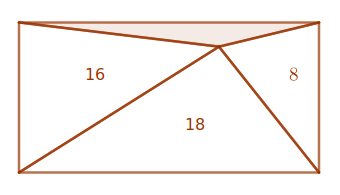
\includegraphics[width=4cm]{./svg/pdf/pi-2024-c-p24.pdf}
    \end{center}

    \[
        (A) \quad 3 \qquad \quad
        (B) \quad 4 \qquad \quad
        (C) \quad 5 \qquad \quad
        (D) \quad 6 \qquad \quad
    \]
\end{problem*}

\begin{soln}
    Chú ý là hai hình tam giac đối diện có cùng đáy, là chiều rộng của hình chữ nhật. Tổng chiều cao của hai hình tam giác bằng chiều cao của hình chữ nhật.
    Do vậy tổng diện tích của hai hình tam giác đối diện sẽ bằng một nữa của chiều rộng nhân chiều cao của hình chữ nhật, tức là một nửa của hình chữ nhật. 
    Do đó diện tích cần tìm là $16 + 8 - 18 = \boxed{6\ (D).}$
\end{soln}

\bigbreak

\begin{problem*}[PI-2024-C-P25]
    \label{problem:pi-2024-c-p25}

    Trong phép nhân bên dưới các chữ cái khác nhau đại diện cho các chứ số khác nhau.
    Các dấu sao đại điên cho bất kỳ một chữ số nào.

    Kết quả của phép nhân là một số có ba chữ số, đó là số nào?

    \begin{center}
        \begin{tabular}{ccc}
                 & A & B \\
        $\times$ & C & B \\ \hline
                 & * & 9 \\
        *        & * &   \\ \hline
        *        & * & *
        \end{tabular}
    \end{center}    

    \[
        (A) \quad 129 \qquad \quad
        (B) \quad 279 \qquad \quad
        (C) \quad 299 \qquad \quad
        (D) \quad 369 \qquad \quad
    \]
\end{problem*}

\begin{soln}
    Tích $B \times B$ tận cùng bằng 9 chỉ khi $B$ là 3 hoặc 7.
    Nếu $B=7$ thì kết quả $A7 \times 7$ phải là một số có ba chữ số, bất kể $A$ là bao nhiêu.
    Do đó $B=3,$ $A=1, C=2$ hoặc $C=1, A=2$ là hai khả năng duy nhất để kết quả là số có ba chữ số nhỏ nhất $13 \times 23 = \boxed{299\ (C).}$
\end{soln}

\bigbreak

\begin{problem*}[PI-2024-C-P26]
    \label{problem:pi-2024-c-p26}

    Hồng Anh nhân 2025 số 2 với 2022 số 5 như sau:
    \[
        \underbrace{2 \times 2 \times \cdots \times 2}_{2025\ \text{số}\ 2} \times \underbrace{5 \times 5 \times \cdots \times 5}_{2022\ \text{số}\ 5}
    \]

    Hỏi chữ số đứng đầu (từ trái qua) của kết quả là bao nhiêu?

    \[
        (A) \quad 1 \qquad \quad
        (B) \quad 2 \qquad \quad
        (C) \quad 4 \qquad \quad
        (D) \quad 8 \qquad \quad
    \]
\end{problem*}

\begin{soln}
    Để ý rằng $2 \times 5 = 10,$ do đó kết quả phép tính sẽ là $2 \times 2 \times 2 \underbrace{10 \times 10 \times \cdots \times 10}_{2022\ \text{số}\ 10}.$
    Dễ thấy rằng chữ số đứng đầu là $\boxed{8\ (D).}$
\end{soln}

\bigbreak

\begin{problem*}[PI-2024-C-P27]
    \label{problem:pi-2024-c-p27}

    Có năm đội sao Hoả và bảy đội sao Kim tham gia Giải vô dịch Bóng đá Liên hành tinh.
    Mỗi đội đấu hai trận với mỗi đội khác hành tinh và đấu một trận với đội cùng hành tinh.
    Hỏi có bao nhiêu trận đấu xảy ra trong toàn giải?

    \[
        (A) \quad 132 \qquad \quad
        (B) \quad 101 \qquad \quad
        (C) \quad 97 \qquad \quad
        (D) \quad 66 \qquad \quad
    \]
\end{problem*}

\begin{soln}
    Các đội sao Hoả thi đấu $5 \times 7 \times 2 = 70$ với các đội sao Kim.
    Các đội sao Hoả thi đấu $\frac{5 \times 4}{2} = 10$ trận với nhau.
    Các đội sao Kim thi đấu $\frac{7 \times 6}{2} = 21$ trận với nhau.
    Tổng số trận là $70+10+21=\boxed{101\ (D).}$
\end{soln}

\bigbreak

\begin{problem*}[PI-2024-C-P28]
    \label{problem:pi-2024-c-p28}

    Chín con khỉ đột nặng bằng bốn con gấu. Tám con gấu nặng ngang mười lăm con báo.
    Mười con báo có trong lượng như hai mươi bảy con nai.
    Hỏi bao nhiêu con nai sẽ nặng như bốn con khỉ đột? 

    \[
        (A) \quad 8 \qquad \quad
        (B) \quad 9 \qquad \quad
        (C) \quad 10 \qquad \quad
        (D) \quad 12 \qquad \quad
    \]
\end{problem*}

\begin{soln}
    Bốn con khỉ đột sẽ nặng như $4 \times \frac{4}{9} = \frac{16}{9}$ con gấu,
    tương đương $\frac{16}{9} \times \frac{15}{8}  = \frac{10}{3}$ con báo,
    tương đương $\frac{10}{3} \times \frac{27}{10}  = \boxed{9\ (B)}$ con nai.
\end{soln}

\bigbreak

\begin{problem*}[PI-2024-C-P29]
    \label{problem:pi-2024-c-p29}

    Ánh và Bình xuất phát cùng một vị trí, cùng thời điểm, và chạy cùng hướng trên một đường chạy thi đấu hình tròn chu vi 200 mét.
    Bình chạy với tốc độ là 5 mét một giây, còn tốc độ của Ánh là 3 mét một giây.

    Hỏi Ánh chạy được bao nhiêu mét khi họ gặp lại nhau lần đầu tiên kể từ khi xuất phát?

    \[
        (A) \quad 200 \qquad \quad
        (B) \quad 300 \qquad \quad
        (C) \quad 400 \qquad \quad
        (D) \quad 600 \qquad \quad
    \]
\end{problem*}

\begin{soln}
    Khi cả hai gặp nhau thì quãng đường Bình chạy hơn so với Ánh là một bội số của chu vi hình tròn.
    Nếu họ chạy đươc $t$ giây thì quãng đường này là $2t.$ Giá trị nhỏ nhất của $t$ để $2t$ là bội số của 200 là $t=100.$
    Lúc này Ánh chạy được $\boxed{300\ (B)}$ mét.
\end{soln}

\bigbreak

\begin{problem*}[PI-2024-C-P30]
    \label{problem:pi-2024-c-p30}

    Một đường tròn chia mặt phẳng thành hai phần.
    Hai đường trờn có thể chia mặt phẳng tối đa thành bốn phần.
    Hai đường trờn có thể chia mặt phẳng tối đa thành tám phần.
    Bốn đường tròn có thể chia mặt phẳng tối đa thành bao nhiêu phần?

    \[
        (A) \quad 13 \qquad \quad
        (B) \quad 14 \qquad \quad
        (C) \quad 15 \qquad \quad
        (D) \quad 16 \qquad \quad
    \]
\end{problem*}

\begin{soln}
    Bốn đường tròn có thể chia mặt phẳng tối đa thành $\boxed{14\ (B)}$ phần như hình bên dưới.
    \begin{center}
        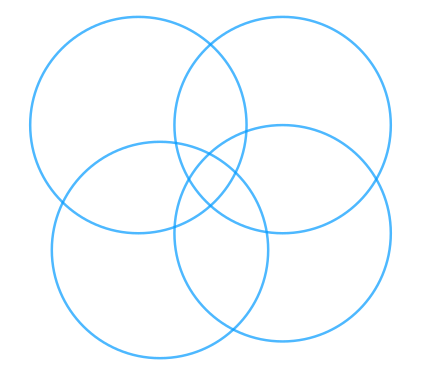
\includegraphics[width=4cm]{./svg/pdf/pi-2024-c-p30.pdf}
    \end{center}
\end{soln}

\end{otherlanguage*}

\end{document}